\documentclass[french]{beamer}

\usepackage[utf8]{inputenc}
\usepackage[T1]{fontenc}
\usepackage{lmodern}
\usepackage{amsmath, amssymb}

\usepackage{babel}
\setbeamertemplate{itemize item}[ball]
\setbeamertemplate{itemize subitem}[triangle]
\setbeamertemplate{itemize subsubitem}[circle]

%CHOIX DU THEME et/ou DE SA COULEUR
% => essayer différents thèmes 
% voir http://mcclinews.free.fr/latex/beamergalerie/completsgalerie.html
\usetheme{PaloAlto}
%\usetheme{Madrid}
%\usetheme{AnnArbor}
%\usetheme{Copenhagen}

% voir http://mcclinews.free.fr/latex/beamergalerie/colorgalerie.html
%\usecolortheme{crane}
%\usecolortheme{seahorse}
%\usecolortheme{albatross}
\usecolortheme{dolphin}
%\useoutertheme[left]{sidebar}


%Pour le TITLEPAGE
\title{Exemple de Beamer}
\subtitle{Initiation master~1}
\author[Nom (court)]{Nom (long) de l'auteur}
\date{Avril 2014}
\institute[UT3 -- FSI]{Université Toulouse~3 -- Faculté des sciences et ingénierie}


\begin{document}

\begin{frame}
	\titlepage
\end{frame}

\begin{frame}
	Un environnement \texttt{frame} pour chaque \emph{diapositive}.
	\visible<2>{Chaque diapo pouvant contenir plusieurs \emph{couches}.}
\end{frame}


\begin{frame}{On peut mettre un titre : Sommaire}
	\tableofcontents
\end{frame}

\section{Exemple}
\begin{frame}{La section 1 commence}
	blabla
\end{frame}

\begin{frame}
	Un \textbf<2,3>{texte} en gras. 
	\visible<3>{Un texte visible sur la 3\ieme{} couche}
\end{frame}

\begin{frame}{Titre (facultatif)} 
\framesubtitle{Sous titre (facultatif aussi)}
	\begin{block}{Remarque}
	Un bloc
	\end{block}
	
	\begin{alertblock}{Proposition}
	Un bloc alerte
	\end{alertblock}
	
	\begin{exampleblock}<2>{Exemple}
	Un bloc exemple qui est visible sur la 2\ieme{} couche : $f(x)=2x$.
	\end{exampleblock}
\end{frame}

\begin{frame}{La section 2 commence}
 voir d'autres exemples dans le dossier exemple.
\end{frame}

\section{Présentation}
\begin{frame}
\tableofcontents[currentsection]
\end{frame}
\begin{frame}
c'est la présentation
\end{frame}

\section{Notre solution : la clé USB}
\begin{frame}
\tableofcontents[currentsection]
\end{frame}

\begin{frame}
  \frametitle{Les Outils}
  \begin{columns}[t]
    \begin{column}{10cm}
      \begin{exampleblock}{Les outils proposés}
	\begin{itemize}
	\item VLC Media Player : un lecteur de média.
	\item Audacity : un éditeur audio.
	\item Metronomix : un métronome.
        \item MuseScore : un éditeur de partition.
	\end{itemize}
      \end{exampleblock} 
    \end{column}
  \end{columns}
  \begin{figure}[!h]
    \centering{
      
\includegraphics[width = 0.15\textwidth]{../images/tool_vlc.png}
      
\includegraphics[width = 0.15\textwidth]{../images/tool_audacity.png}
      
\includegraphics[width = 0.15\textwidth]{../images/tool_metronomix.png}
      
\includegraphics[width = 0.15\textwidth]{../images/tool_score.png}
    }
    \label{VLC, Audacity, Metronomix et MuseScore} 
    \caption{VLC, Audacity, Metronomix et MuseScore}
  \end{figure}        
\end{frame}

\begin{frame}
  \frametitle{Le Quizz}
  Le Quizz est composé de 2 écrans :
  \begin{columns}[t]
    \begin{column}{10cm}
      \begin{exampleblock}{L'écran de selection}
	\begin{itemize}
        \item Choix du thème.
        \item Choix de la difficulté.
        \end{itemize}
      \end{exampleblock} 
    \end{column}
  \end{columns}  

  \begin{columns}[t]
    \begin{column}{10cm}
      \begin{exampleblock}{L'écran de quizz}
	\begin{itemize}
        \item Question au format texte, image ou son.
        \item Réponse à choix multiples.
        \item Explication du professeur.
        \item Temps limité.
        \end{itemize}
      \end{exampleblock} 
    \end{column}
  \end{columns}  
\end{frame}

\begin{frame}
  \frametitle{Le Jeu}
  Le jeu s'inspire du classique \textbf{Space Invaders}.
  \begin{itemize}
    \item Le joueur contrôle un vaisseau qui doit attaquer des notes de musique.    \item La note à attaquer change régulièrement.
    \item La difficulté augmente en fonction du cursus musical des élèves.  
  \end{itemize}

  \begin{figure}[!h]
    \centering
    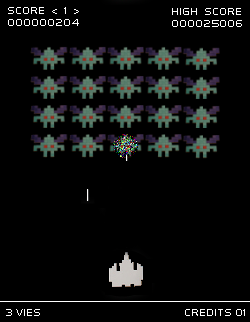
\includegraphics[height = 0.5\textheight]{img/Space_Invaders.png}
    \label{Space Invaders} 
    \caption{Space Invaders}
  \end{figure}
\end{frame}

\begin{frame}
  \frametitle{Administration et aide}
 \begin{columns}[t]
    \begin{column}{10cm}
      \begin{exampleblock}{Les différents menus}
	\begin{itemize}
        \item Un menu qui permet de modifier les données du quizz ou du jeu.
        \item Choix de la langue.
        \item Aide pour l'utilisateur.
        \end{itemize}
      \end{exampleblock} 
    \end{column}
  \end{columns}  
\end{frame}

\begin{frame}

\end{frame}
\section{Organisation}

\begin{frame}
\tableofcontents[currentsection]
\end{frame}
\begin{frame}
lorem lipsum
\end{frame}
\begin{frame}
 
\end{frame}
\section{Conception et développement}

\begin{frame}
\tableofcontents[currentsection]
\end{frame}
\begin{frame}
lorem lipsum
\end{frame}
\begin{frame}
 
\end{frame}
\section{Problèmes rencontrés}

\begin{frame}
\tableofcontents[currentsection]
\end{frame}
\begin{frame}
lorem lipsum
\end{frame}
\begin{frame}
 
\end{frame}
\section{Perspectives d'évolution}

\begin{frame}
\tableofcontents[currentsection]
\end{frame}
\begin{frame}
lorem lipsum
\end{frame}
\begin{frame}
 
\end{frame}
\input{bonus_track.tex}


\end{document}